\documentclass[12pt]{article} % Tamaño de letra
\usepackage[utf8]{inputenc} % Simbolo utf8
\usepackage[light]{antpolt} % Tipo de letra
\usepackage[T1]{fontenc}
\usepackage[spanish]{babel} % Español 
\usepackage[dvipsnames]{xcolor} % Paquete de colores
\usepackage{amsmath} % Paquete de simbolos matematicos
\usepackage{halloweenmath} % Paquete de Halloween
\usepackage{amssymb} % therefore 
\usepackage{amsfonts}  % Alinear
\usepackage{mathtools} 
\usepackage{hyperref} % Hiperreferencias
\usepackage{xurl} % Romper url largos en más líneas
\usepackage{graphicx}
\usepackage{caption} % Paquete para personalizar las captions
\usepackage{tikz} % Dibujos arreglo
\usepackage{graphics}
\usepackage{wrapfig}
\usepackage{subfig}
\usepackage{listings} % Código
\usepackage[shortlabels]{enumitem}
\usepackage{bbm}
\usepackage{multirow, array} % para las tablas
\usepackage{float}
\usepackage{color}
\usepackage{tabularray}
\usepackage{fancyhdr}
\usepackage{pifont}%Simbolos especiales.
\usepackage{fancybox}%Para crear cajas (Notas).
\usepackage[margin=1in]{geometry}
\usepackage[margin=1.1in]{caption}
\pagestyle{fancy}
\fancypagestyle{plain}{
\fancyhf{}\fancyhead[L]{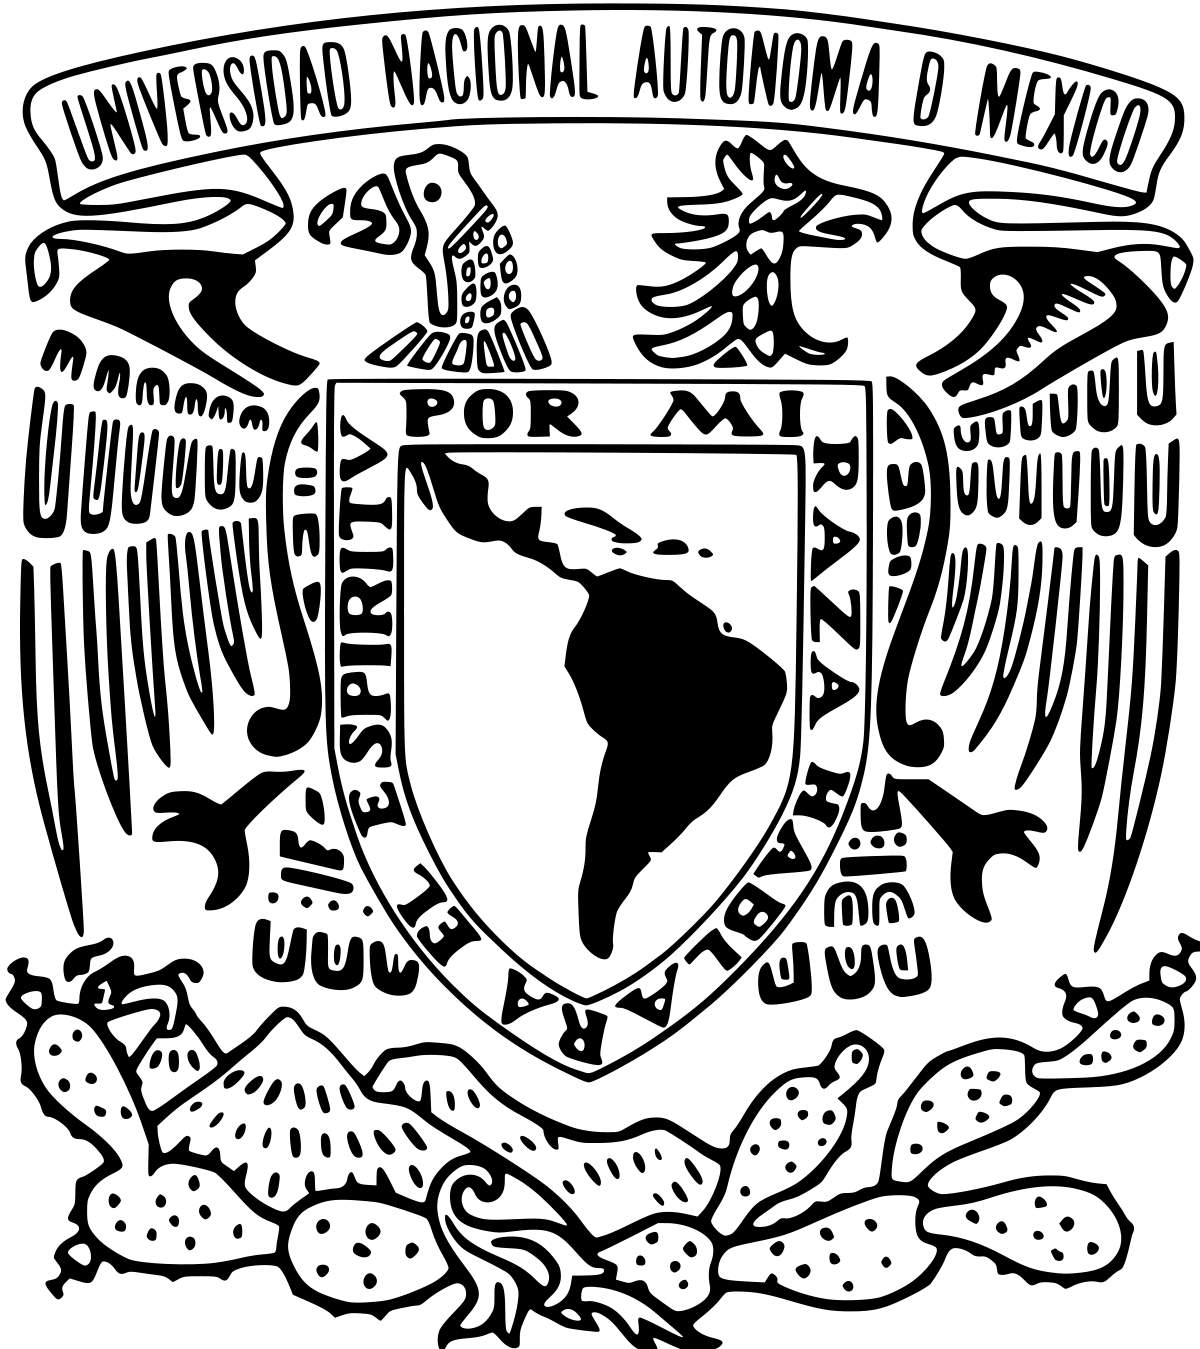
\includegraphics[height=0.5in]{unam.png}}
\fancyhead[R]{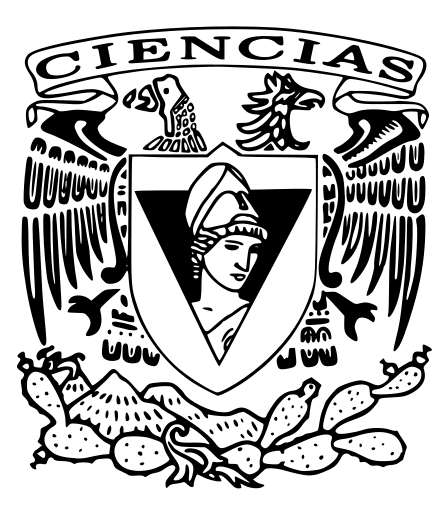
\includegraphics[height=0.5in]{ciencias.png}}
}

%----------[ Declaración Respuesta ]-----------
\usepackage{framed,xcolor} % Color de repuesta

\newenvironment{respuesta}{
    \definecolor{shadecolor}{RGB}{236,236,228}
    \begin{snugshade*}
    \vspace*{2mm}}
    {\vspace*{2mm}
    \end{snugshade*}}

%------------------------------
\definecolor{fondo}{RGB}{234, 236, 238}% Definición del color fondo

\lstset{
    language=Java,
    basicstyle=\ttfamily\footnotesize, % Cambiar el tamaño de la fuente
    keywordstyle=\color{blue},
    commentstyle=\color{OrangeRed},
    stringstyle=\color{ForestGreen},
    numbers=left,
    numberstyle=\tiny,
    stepnumber=1,
    numbersep=5pt,
    backgroundcolor=\color{fondo},
    frame=single,
    rulecolor=\color{black},
    breaklines=true,
    columns=flexible,
    inputencoding=utf8,
    morecomment=[s][\color{purple}]{/**}{*/},
    %morecomment=[l][\color{orange}]{//},
    %literate={\#}{{\#}}1,
    literate={á}{{\'a}}1
             {é}{{\'e}}1
             {í}{{\'i}}1
             {ó}{{\'o}}1
             {ú}{{\'u}}1
             {Á}{{\'A}}1
             {É}{{\'E}}1
             {Í}{{\'I}}1
             {Ó}{{\'O}}1
             {Ú}{{\'U}}1
             {ñ}{{\~n}}1
             {Ñ}{{\~N}}1
             {¿}{{\textquestiondown}}1
             {¡}{{\textexclamdown}}1,
}

\begin{document}
\title{Ejercicios 2: Complejidad Computacional}
\author{Ayudante: Cynthia Lizbeth Sánchez Urbano}
\date{Ejercicios de práctica para calcular la complejidad basándose en el código.}
\maketitle
\begin{enumerate}
\item Observa el siguiente código:
\begin{lstlisting}
public void imprimePares(int n) {
    for (int i = 0; i < n; i++) {
        if (i % 2 == 0) {
            System.out.println(i);
        }
    }
}
\end{lstlisting}
¿Cuál es la complejidad del algoritmo en tiempo y por qué?
¿Cuál es la complejidad del algoritmo en espacio y por qué?
\item
\begin{lstlisting}
public void buscaAlumno(String nombre) {
    String[] arreglo = { "Anna Sánchez", "Julio Lozano", ..., "Óscar López"};
    for (String s : arreglo)
        if (s.equals(nombre)) {
            System.out.println(s + " encontrado");
            return;
        }
    System.err.println("Alumno no encontrado");
}
\end{lstlisting}
¿Cuál es la complejidad del algoritmo en tiempo y por qué?
¿Cuál es la complejidad del algoritmo en espacio y por qué?
\item
\begin{lstlisting}
 public int[] bubbleSort(int[] arreglo) {
     for (int i = 1; i < arreglo.length; i++) {
          for (int j = 0; j < arreglo.length - i; j++) {
               if (arreglo[j] > arreglo[j + 1]) {
                   int temp = arreglo[j];
                   arreglo[j] = arreglo[j + 1];
                   arreglo[j + 1] = temp;
               }
          }
     }
     return arreglo;
}
\end{lstlisting}
¿Cuál es la complejidad del algoritmo en tiempo y por qué?
¿Cuál es la complejidad del algoritmo en espacio y por qué?
\item 
\begin{lstlisting}
  public static int factorial(int n) {
      if (n < 0) {
          throw new IllegalArgumentException("El número debe ser positivo");
      }
      return auxFactorial(n);
  }

  public static int auxFactorial(int n) {
      if (n == 0) {
          return 1;
      }
      return n * auxFactorial(n - 1);
  }
\end{lstlisting}
¿Cuál es la complejidad del algoritmo en tiempo y por qué?
¿Cuál es la complejidad del algoritmo en espacio y por qué?
\item
\begin{lstlisting}
  public static double promedio(double[] arreglo) {
      double suma = 0;
      for (double i : arreglo) {
           suma += i;
      }
      return suma / arreglo.length;
  }
\end{lstlisting}
¿Cuál es la complejidad del algoritmo en tiempo y por qué?
¿Cuál es la complejidad del algoritmo en espacio y por qué?
\end{enumerate}
\end{document}